
%(BEGIN_QUESTION)
% Copyright 2010, Tony R. Kuphaldt, released under the Creative Commons Attribution License (v 1.0)
% This means you may do almost anything with this work of mine, so long as you give me proper credit

Suppose we have an Allen-Bradley MicroLogix 1000 PLC and two pressure switches we need to connect to it:

$$\includegraphics[width=15.5cm]{i04639x01.eps}$$

Determine the necessary contacts on each pressure switch (NO versus NC) we need to connect to the PLC inputs in order to make the lamp turn on when pressure A exceeds 25 PSI and pressure B drops below 139 PSI, given the following program running in the PLC:

$$\includegraphics[width=15.5cm]{i04639x02.eps}$$

\underbar{file i04639}
%(END_QUESTION)





%(BEGIN_ANSWER)

Both pressure switches need their {\it normally-closed} (NC) contact terminals connected to the respective PLC input terminals.

%(END_ANSWER)





%(BEGIN_NOTES)


%INDEX% PLC, relating I/O status to virtual elements 

%(END_NOTES)


